\section{Hardware laget og konfiguration af periferienheder}
I det kommende afsnit vil den valgte hardware konfiguration blive gennemgået. 
Den dybere tekniske beskrivelse i forhold til fx. produkt specifikke registre eller anden speciel arkitektur, vil ikke i detaljer blive beskrevet, medmindre det er en vigtig del af argumentationen for valget.
Det komplette hardware modul findes i \emph{hardware.c}.

\subsection{Valg af hardware profil}
For at kunne håndtere de forskellige opsætninger af hardware i udviklingsforløbet af equalizerens software, er der lavet forskellige hardware opsætninger, således at det er nemt kan skiftes mellem dem.
\\

I \textit{global.h} filen, findes to compilere \textbf{\#define} direktiver til makro definitionerne \texttt{EMP} og \texttt{DAC}.
Sammenhængen mellem profilerne ses i figur \ref{fig:hardware_profiler}. 
Softwaren kan således testes på EMP printet\footnote{Komponenterne til mikrofonindgang og hovedtelefonudgang skal være monteret \cite{emp-diagram}.}, ved at vælge \texttt{EMP} profilen.
Fravælges \texttt{EMP} profilen, skifter softwaren over til at bruge projekt printet.
Her kan der vælges imellem DAC eller PWM som udgangssignal.  
Den tilhørende pin-konfiguration for de valgte hardware profiler kan ses i bilag \ref{bilag:pinmap}.

\subsection{CPU'ens clock frekvens}
\begin{wrapfigure}[20]{r}{5cm}
	\centering
	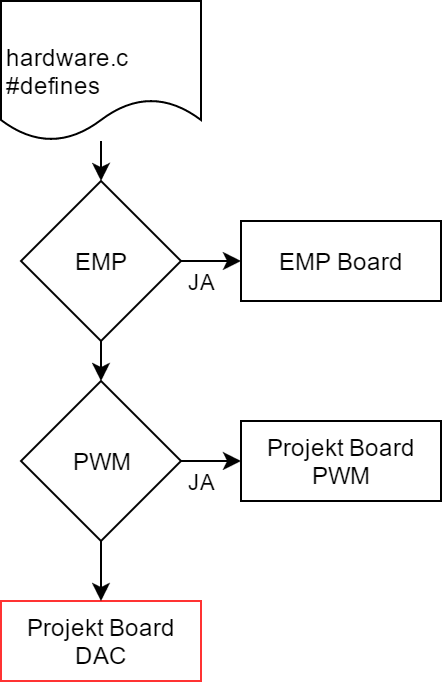
\includegraphics[width=4.5cm]{billeder/hardware_profiles.png}
	\caption{Oversigt over mulige konfigurationer af \textit{hardware.c}.}
	\label{fig:hardware_profiler}
\end{wrapfigure}
For at kunne opnå så mange beregninger som muligt i sekundet, opsættes MCU'en til den maksimale clock frekvens.
Den valgte MCU (TM4C123GH6PM) er en $80\si{\mega\hertz}$ mikrokontroller, og den ønskede clock frekvens sættes i funktionen \texttt{set\_80Mhz\_clock();} i hardwaremodulet \textit{hardware.c} til $F_{CPU} = 80\si{\mega\hertz}$.\\
Ved denne frekvens og den valgte samplefrekvens $F_s$, kan et mål for antallet af CPU cycles imellem hver sample findes.
\begin{align}
N_{CPU cycles} = \frac{F_{CPU}}{F_s}  =  \frac{80\si{\mega\hertz}}{44,1\si{\kilo\hertz}}  = 1814,06 \si{\cycles}
\end{align}

\subsection{ADC}\label{subsec:adc}
Til sampling af lydsignalet anvendes en analog til digital konverter (ADC). 
De tre vigtigste faktorer der skal findes frem til er - hvornår der bliver samplet, hvor længe det varer før værdien er tilgængelig og hvor nøjagtig den den samplede værdi er.\\

ADC'en omsætter det analoge lydsignal til en digital repræsentation, i dette tilfælde med en 12 bits opløsning\footnote{Stadard ADC opløsning på \textit{M4C123GH6PM} MCU'en \cite[s. 797]{tm4c123gh6pm}}.\\
Opløsningen på det indgående lydsignal kan bestemmes til $V_{LSb} = (V_{ref+} - V_{ref-} ) / 4096 $, hvor $V_{ref+}$ og $V_{ref-}$ er henholdsvis den positive og negative referencespænding.
I den konkrete løsning, forsynes MCU'en med en single-supply på $V_{DD} = 3,3\si{\volt}$.
Derved bliver den mindste målbare spændingsændring på indgangen,
\begin{align}
V_{LSb} = \frac{V_{DD}}{4096} = 8,06\si{\milli\volt\per\LSb}
\end{align}

For et komplet billede af nøjagtigheden på det samplede signal, fremgår det i databladet \cite[afsnit 24.14 s. 1383]{tm4c123gh6pm} for MCU'en, at
den samlede, ikke korrigerede maksimale fejl er $E_T = \pm 30\si{\LSb}$.

Den samplede digitale spænding $V_{d}$, kan således angives med en usikkerhed i forhold til den analoge spænding $V_{a}$ på,
\begin{align}
V_{d} = V_{a} \pm \V_{LSb} \cdot E_T = V_{a} \pm   8,06\si{\milli\volt\per\LSb} \cdot 30 \si{\LSb} = V_{a} \pm 24,17\si{\milli\volt}
\end{align} 

Den i projektet anvendte MCU tilbyder en lang række funktionaliteter for ADC periferienheden.
Det er dog kun nødvendigt at fortage én lydsampling for hver lyd kanal\footnote{Når software anvender EMP profil bruges der kun én ADC kanal}, én gang for hver sampleperiode $T_s$.
Derfor anvendes en \textbf{Once Mode}\cite[afsnit 13.3.7.2, s. 812]{tm4c123gh6pm}, der bliver styret af interrupt service rutinen \texttt{sample\_handler();}. Denne ISR og timingen af ADC'en vil blive uddybet i afsnittet om interrupt (se side \pageref{subsec:interrupt}).\\

Samplingen ved ADC'en på lydsignalet påbegyndes manuelt af equalizerens software.
ADC'en bruger successiv approksimation (SAR) og ud fra databladet er sampletiden angivet som $T_C = 2$ ADC clock cycles. 
Implementeringen af ADC har en clock-frekvens sat til $16 \si{\mega\hertz}$ som giver en samplingstid på $T_C = \num{1,25E-7}\si{\second}$.  

\subsection{PWM - Pulse Width Modulation}\label{subsec:pwm}
I begyndelsen af udviklingen, var der overvejelser om hvordan lydsignalet skulle genskabes efter den digitale behandling var foregået.
Ud fra de indbyggede periferienheder, som den valgte MCU stiller til rådighed, faldt valget på et PWM genereret lydsignal.
Det viste sig dog under udviklingen af de analoge filtre ( som blev gennemgået i foregående kapitel ), at en tilfredsstillende lydkvalitet samt at kunne eftervise equalizerens funktionalitet, ikke kunne opnås med et PWM generet lydsignal. \\
Der vil dog stadig laves en gennemgang af PWM'ens opsætning og funktionalitet i hardware delen, da denne bruges i \texttt{EMP} profilen.\\

Som udgangspunkt er det anvendte EMP print udstyret med en mikrofonindgang og en hovedtelefonudgang \footnote{Henholdsvis \textbf{Microphone Preamp} og \textbf{Headphone Output} i diagram \cite{emp-diagram}}. Disse er fra designerens side, blevet forbundet med henholdsvis en af MCU'ens analoge indgange og en GPIO pin hvor PWM er mulig\footnote{Forbindelserne kan ses i \cite{emp-diagram} og i pinmapping tabellen i bilag \ref{bilag:pinmap}}.

\begin{figure}[h!]
	\centering
	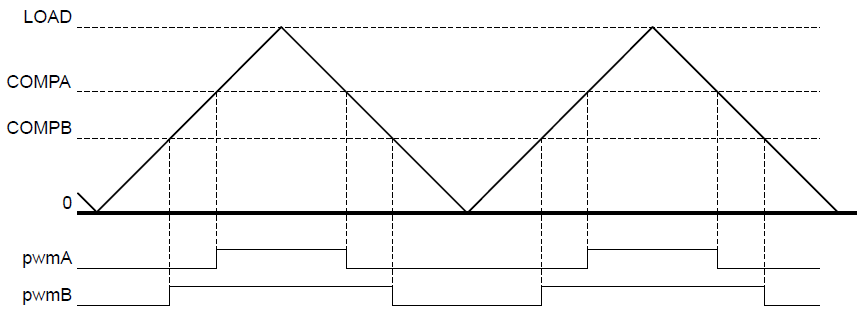
\includegraphics[width=.7\textwidth]{billeder/pwm.png}
	\caption{Eksempel på PWM generator i MCU'en for i fase korrekt modus eller \textbf{Count-Up/Count-down mode}\cite[Fig. 20-5 s. 1232]{tm4c123gh6pm}.}
	\label{fig:pwm}
\end{figure}

Der vælges at bruge PWM i fase korrekte modus, hvor et eksempel ses i figur \ref{fig:pwm}.
I fasekorrekt modus skal PWM tælleren starte på 0 og tælle både op til \textbf{LOAD} værdien og ned igen, inden næste PWM cyklus påbegyndes.
Ved en PWM frekvens $F_{PWM}$, der er den samme som samplingsfrekvensen $F_s$, vil $\textbf{LOAD} = N_{CPU cycles} / 2$.

Da udgangssignalet kan variere mellem $ 0 \si{\volt}$ og $V_{DD} = 3,3 \si{\volt}$, hvor middelværdien er $V_{DD}/2 = 1,65 \si{\volt}$, kan opløsningen på udgangssignalet beregnes til.

\begin{align}
\Delta V_{PWM} = \frac{V_{DD} \cdot 2K}{N_{CPU cycles}} = \frac{3,3\si{\volt} \cdot 2}{1814} =  3,638\si{\milli\volt}
\end{align}

Her angiver $K$ et vilkårligt forhold mellem samplingsfrekvens og PWM frekvens.\\

Da der ønskes en PWM frekvens der er 10 gange større end samplingsfrekvensen $[K=10]$ ses det, at opløsningen på udgangen ligeledes falder med en faktor 10 til $\Delta V_{PWM} = 36,38\si{\milli\volt}$.\\

Det er således ikke hensigtsmæssigt at anvende et PWM genereret lydsignal på udgangen.
Derfor blev der sidste i udviklingen skiftet til en DAC som der kommes nærmere ind på i næste afsnit.\\

Opsætning af PWM findes i \texttt{init\_PWM( INT16U cycles );} i hardware modulet \textit{hardware.c}. 
Funktionen tager $N_{CPU cycles}$ som parameter, således at hardwaren kan opsættes til andre samplingsfrekvenser end $F_s = 44,1\si{\kilo\hertz}$.
Afhængig af den valgte hardware profil, sættes pin konfigurationen ud fra tabellen i bilag \ref{bilag:pinmap}.  

\FloatBlock

\subsection{DAC}
Til at generere udgangssignalet fra MCU'en vælges en ekstern DAC kreds, da MCU'en ikke råder over denne funktionalitet.
Valget blev en \texttt{MCP4922E/P}\footnote{Microchip MCP4922E/P 12-Bit Dual Voltage Output Digital-to-Analog Converter with SPI Interface \cite{mcp4922} } som er en 12bit DAC IC.
Derved er opløsningen på udgangen den samme som på indgangen (se afsnit om ADC på side \pageref{subsec:adc}).\\

Spændingsdifferencen vil for den mindst betydende bit være $ V_{LSb} = V_{ref} / 4096 \approx \num{0,8}\si{\milli\volt} $, ved en ekstern reference spænding på $V_{ref} = 3,3\si{\volt}$.
Derudover har den valgte DAC en maksimal indsvingningstid på $t_{settling} = \num{4.5}\si{\micro\second}$, hvilket passer fint til samplingsperioden på $T_s = 23\si{\micro\second}$. 

\subsection{SPI}
Den valgte DAC forbindes direkte til MCU'en gennem en SPI bus, hvor de valgte pins er beskrevet i bilag \ref{bilag:pinmap}.
Ifølge databladet er datakommunikation op til $20\si{\mega\hertz}$ mulig, men SPI port konfigurationen på MCU'en sættes til $10\si{\mega\hertz}$.
For at sætte den ønskede udgangsspænding på DAC'en, er en 16 bit kommando nødvendig\footnote{En komplet beskrivelse af SPI protokollen findes i \cite[s. 23]{mcp4922}.}. 
I figur \ref{fig:dac12bit_writecmd} ses den nødvendige kommando-bitsekvens med tilhørende timingsdiagram for \textbf{CS}, \textbf{SCK} og \textbf{LDAC}  .\\

En SPI clock på $F_{SCK} = 10\si{\mega\hertz}$, giver således en transmissionstid $t_{cmd}$ af SPI kommandoen for begge lydkanaler på minimum på 
\begin{align}
	t_{cmd} = \frac{N_{kanal} \cdot 16bit}{F_{SCK}} = \frac{2 \cdot 16}{10\si{\mega\hertz}} = 3\si{\micro\second}
\end{align}

\begin{figure}[h!]
	\centering
	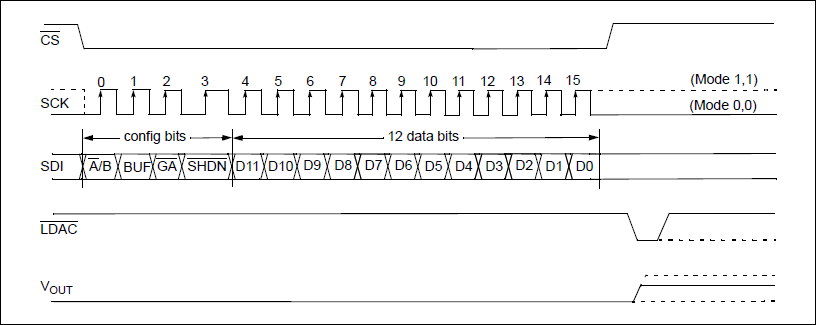
\includegraphics[width=.8\textwidth]{billeder/dac12bit_writecmd.png}
	\caption{Skrive kommando til 12bit MCP4922 DAC.\cite[s. 25]{mcp4922}}
	\label{fig:dac12bit_writecmd}
\end{figure}

I overensstemmelse med databladene for DAC'en og MCU'en, bruges \emph{SPI Freescale Fame} formatet\footnote{Se afsnit 15.3.4 \cite[s. 954]{tm4c123gh6pm}} i \textbf{Mode 0,0}.

\begin{figure}[h!]
	\centering
	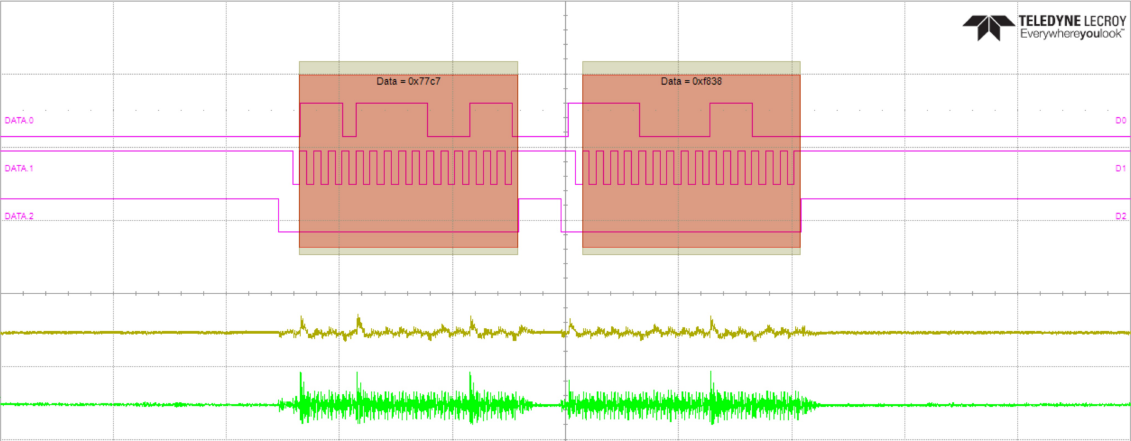
\includegraphics[width=\textwidth]{billeder/dac_dataframe.png}
	\caption{(Øverst) Dataframe til DAC. \textit{Data.0} = SDI, \textit{Data.1} = SCK, \textit{Data.2} = CS - Signal før (Grøn) og efter (Gul)  $1\si{\mega\hertz}$ udgangsfilter - $1.00\si{\micro\second}\text{/Div}$}
	\label{fig:dac_dataframe}
\end{figure}

Konfigurationen af SPI findes i \texttt{spi\_init();} i modulet \textit{hardware.c}  

\FloatBlock

\subsection{Interrupt}\label{subsec:interrupt}
Som det tidligere er blevet forklaret, er der et kald til \texttt{sample\_handler();} ISR'en der ligger til grund for hele timingen af lydsamplingen.
Det er dog ikke vigtigt hvilken interrupt vektor der får denne opgave.\\

I dette system er der valgt at bruge \textbf{zero reload event} på PWM'en, som \textit{interrupt trigger}.
Således bliver samplingstiden, som PWM'en er sat op efter (se afsnit om PWM på side \pageref{subsec:pwm}), indirekte overført til både ADC'en og DAC'en.\\ 

Konfiguration af \textbf{NVIC}'en kan findes i modulet \textit{tm4c123gh6pm\_startup\_ccs\_gcc.c} og funktionen \texttt{init\_PWM(INT16U cycles);} i hardware modulet \textit{hardware.c}

\subsection{UART}\label{subsec:uart}
Det er muligt at tilgå Shell'en i equalizeren via seriel kommunikation.
I task modellen (figur \ref{fig:eq-taskmodel}) ses kommunikationen mellem \textbf{UART RX/TX} task'ene og Shell tasken.
Grundet hastighedsforskellen imellem scheduleringen af shell'en tasken og den meget langsommere serielle kommunikation, er \textbf{RX/TX queues} implementeret med asymmetrisk størrelse. 	
\textbf{TX queue} er således 1KB og \textbf{RX queue} er kun  250 bytes.

Standard opsætningen for seriel kommunikation er
\begin{center}
	\textbf{Baudrate : }19200  \quad \textbf{Databits : } 8 \quad \textbf{Stopbits : }1
\end{center}

Opsætningen af UART'en findes i \texttt{uart0\_init(...);} i uart modulet \textit{uart.c}

\subsection{LCD}
LCD displayet der er monteret på EMP printet, er primært brugt under udvikling til at vise debug information. På samme måde bliver det derfor  brugt på projekt printet.
Information som VU-meter, equalizerens tilstand, valgt equalizer profil navn, CPU belastning samt en simpel repræsentation af equalizerens frekvens spektrum kan aflæses på LCD displayet.\\

LCD modulet er sammensat af et driver API sammen med en \texttt{LCD\_buffer\_task(...);} der sørger for at opdatere selve LCD'en.
Skrivning til LCD displayet sker ikke direkte, da API'et skriver i en shared-memory buffer, som bliver brugt af LCD buffer tasken, se figur \ref{fig:eq-taskmodel}.\\
 
I figur \ref{fig:lcd_task} ses state diagrammet for LCD tasken. State variablen er en direkte afspejling af offset positionen i memory bufferen. \textbf{State N} repræsenterer alle de mellemliggende states.

\begin{figure}[h!]
	\centering
	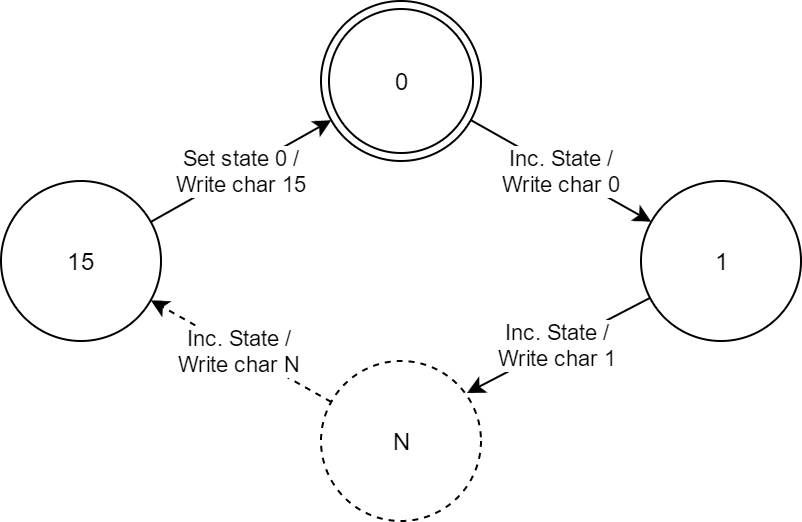
\includegraphics[width=.6\textwidth]{billeder/lcd_task.png}
	\caption{LCD buffer task state diagram.}
	\label{fig:lcd_task}
\end{figure}

LCD displayet bliver initialiseret fra modulet \textit{emp\_lcd1602.c} i  \texttt{lcd\_init();}
  
\FloatBlock

\subsection{Tiva™ C Series TM4C123G LaunchPad Evaluation Board}
Som udviklingsplatform anvendes Tiva LaunchPad \cite{spmu296}. 
Tiva LaunchPad stiller en række funktionaliteter til rådighed som f.eks. On-board ICDI\footnote{(ICDI) In-Circuit Debug Interface (Eng.)}.
Derudover er der på printet også monteret 2 trykknapper (\textbf{SW1 / SW2}) og en RGB LED, som er medtaget i pin mapping tabellen i bilag \ref{bilag:pinmap}, således at det ikke påvirker hardwareprofilen til projektet.   

\subsection{FPU}
For at kunne gøre brug af FPU'en (floating point unit) på den valgte MCU, kræver den en produkt specifik aktivering.
Ifølge \cite[afsnit 3.1.5.7 s. 132]{tm4c123gh6pm} er den implementeret som følgende i hardware modulet \textit{hardware.c}.

\lstset{language=C,
	frame=sigle,
	basicstyle=\ttfamily\tiny,
	emph={INT32U,NVIC_CPAC_R},
	emphstyle={\color{blue}},
	keepspaces=true,
	frame=single,
%	numbers=left,
%	numbersep=5pt,
	numberstyle=\tiny\color{black},
	keywordstyle=\color{red}\ttfamily,
	stringstyle=\color{blue}\ttfamily,
	commentstyle=\color{OliveGreen}\ttfamily,
	morecomment=[l][\color{magenta}]{\#}
}
\begin{tabular}{l}
\begin{lstlisting}[title=init\_FPU()]
INT32U reg;
reg = NVIC_CPAC_R;    // Coprocessor Access Control (CPAC) register
reg |= (0xF << 20);   // Set bits 20-23 to enable 
NVIC_CPAC_R = reg;    // 	CP10 and CP11 coprocessors

__asm__("DSB");       // Data Synchronisation Barrier
__asm__("ISB");       // Instruction Synchronisation Barrier
\end{lstlisting}
\end{tabular}

%\subsection{Timers og sysTick}

 